\documentclass[12pt, a4paper]{article}

% --- PACKAGES ---
\usepackage[utf8]{inputenc}
\usepackage[english]{babel}
\usepackage{geometry}
\usepackage{graphicx}
\usepackage{amsmath}
\usepackage{tikz}
\usepackage{pgfplots}
\usepackage{hyperref}
\usepackage{fancyhdr}
\usepackage{booktabs} % For professional tables
\usepackage{listings} % For MATLAB code

% --- PAGE GEOMETRY & HEADERS ---
\geometry{a4paper, margin=2.5cm}
\pagestyle{fancy}
\fancyhf{}
\fancyhead[L]{Electrical Lines and Distribution Networks}
\fancyhead[R]{University of Almería}
\fancyfoot[C]{\thepage}
\renewcommand{\headrulewidth}{0.4pt}

% --- TIKZ & PGFPLOTS LIBRARIES AND SETTINGS ---
\usetikzlibrary{shapes.geometric, arrows.meta, positioning, calc}
\pgfplotsset{compat=1.18}

% --- MATLAB CODE LISTING STYLE ---
\definecolor{codegreen}{rgb}{0,0.6,0}
\definecolor{codegray}{rgb}{0.5,0.5,0.5}
\definecolor{codepurple}{rgb}{0.58,0,0.82}
\definecolor{backcolour}{rgb}{0.95,0.95,0.92}

\lstdefinestyle{mystyle}{
    backgroundcolor=\color{backcolour},   
    commentstyle=\color{codegreen},
    keywordstyle=\color{blue},
    numberstyle=\tiny\color{codegray},
    stringstyle=\color{codepurple},
    basicstyle=\footnotesize\ttfamily,
    breakatwhitespace=false,         
    breaklines=true,                 
    captionpos=b,                    
    keepspaces=true,                 
    numbers=left,                    
    numbersep=5pt,                  
    showspaces=false,                
    showstringspaces=false,
    showtabs=false,                  
    tabsize=2
}
\lstset{style=mystyle}

% --- DOCUMENT METADATA ---
\title{
    \vspace{2cm}
    \textbf{Technical Report: Week 3 \\ Network Topology Analysis and Design} \\
    \large{Block 2: Electrical Lines and Distribution Networks}
    \vspace{3cm}
}
\author{Student C: Commercial Center Project}
\date{October 15, 2025}


% =================================================================
% --- DOCUMENT START ---
% =================================================================
\begin{document}

% --- PAGE 1: TITLE PAGE ---
\begin{titlepage}
    \maketitle
\end{titlepage}
\thispagestyle{empty}

% --- PAGE 2: TABLE OF CONTENTS ---
\newpage
\tableofcontents
\thispagestyle{empty}
\newpage

\pagestyle{fancy} % Reactivate fancy page style after title and ToC

% =================================================================
\section{Analysis of Radial Distribution Networks}
\subsection{Theoretical Framework}
A radial distribution network is the simplest and most economical topology. It is characterized by a single power path from the substation to the end consumers. The network branches out like a tree, with power flowing in only one direction—from the source outwards. Its main advantages are low initial cost and simplicity in planning and operation. However, its significant disadvantage is low reliability; a single fault on a main feeder will interrupt service for all downstream customers.

\subsection{Design and Calculation Methods}
The design of a radial network is governed by two primary constraints: ensuring the voltage drop at the furthest consumer remains within statutory limits (typically 3-5\% in LV networks) and ensuring that the current in any section does not exceed the conductor's thermal limit (maximum admissible current).

The calculation is performed sequentially, starting from the source. For each segment between nodes, the power flow, resulting current, and voltage drop are calculated. The total voltage drop at any point is the cumulative sum of the drops in all preceding segments.

\subsection{Unifilar Diagram and Characteristic Profiles}
The structure and behavior of a radial network can be visualized through its unifilar diagram and its voltage/current profiles.

\begin{figure}[htbp]
    \centering
    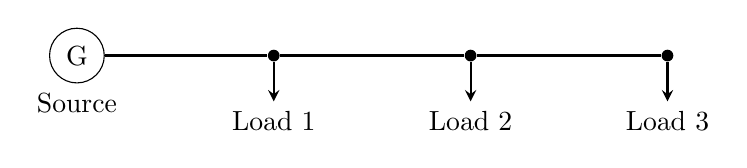
\begin{tikzpicture}[
        node distance=2.5cm,
        bus/.style={fill, circle, inner sep=1.5pt},
        load/.style={-stealth, thick},
        line/.style={thick}
    ]
        % Nodes
        \node[draw, circle, label=below:Source] (source) {G};
        \node[bus, right of=source] (bus1) {};
        \node[bus, right of=bus1] (bus2) {};
        \node[bus, right of=bus2] (bus3) {};
        
        % Lines
        \draw[line] (source.east) -- (bus1);
        \draw[line] (bus1) -- (bus2);
        \draw[line] (bus2) -- (bus3);
        
        % Loads
        \node[below=0.5cm of bus1] (load1_label) {Load 1};
        \draw[load] (bus1) -- (load1_label.north);
        \node[below=0.5cm of bus2] (load2_label) {Load 2};
        \draw[load] (bus2) -- (load2_label.north);
        \node[below=0.5cm of bus3] (load3_label) {Load 3};
        \draw[load] (bus3) -- (load3_label.north);
    \end{tikzpicture}
    \caption{Unifilar diagram of a general radial distribution network.}
    \label{fig:radial_diagram}
\end{figure}

\begin{figure}[htbp]
    \centering
    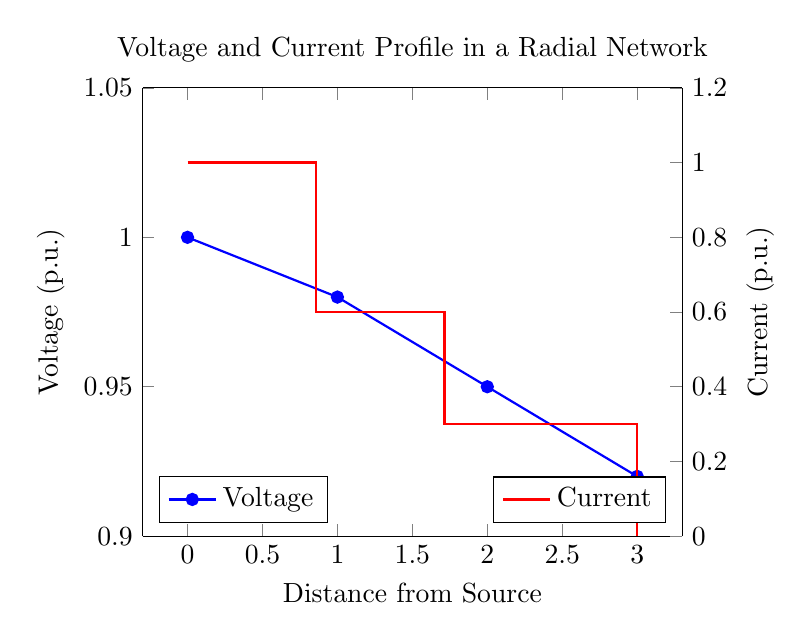
\begin{tikzpicture}
        \begin{axis}[
            title={Voltage and Current Profile in a Radial Network},
            xlabel={Distance from Source},
            ylabel={Voltage (p.u.)},
            ymin=0.9, ymax=1.05,
            axis y line*=left,
            legend pos=south west
        ]
            \addplot[blue, thick, mark=*] coordinates {(0, 1.0) (1, 0.98) (2, 0.95) (3, 0.92)};
            \addlegendentry{Voltage}
        \end{axis}
        \begin{axis}[
            ylabel={Current (p.u.)},
            ymin=0, ymax=1.2,
            axis y line*=right,
            axis x line=none,
            legend pos=south east
        ]
            \addplot[red, thick, const plot] coordinates {(0, 1.0) (1, 0.6) (2, 0.3) (3, 0.3) (3.5,0)};
            \addlegendentry{Current}
        \end{axis}
    \end{tikzpicture}
    \caption{Voltage steadily decreases with distance, while current drops in steps as loads are served.}
    \label{fig:radial_profiles}
\end{figure}

% =================================================================
\section{Analysis of Networks Fed from Both Ends}
\subsection{Theoretical Framework}
Feeding a distribution line from two sources significantly enhances its performance. This topology improves voltage regulation, increases reliability, and doubles the power delivery capacity compared to a similar radial line. Power flows from both ends towards a point of minimum voltage, known as the division point. If one source fails, the other can still supply all loads, albeit with a larger voltage drop.

\subsection{Design and Calculation Methods}
The key challenge in analyzing this network is to determine the division point, where the current supplied from one source meets the current from the other. This can be found by applying superposition or by writing Kirchhoff's voltage law for the loop and solving for the point where current is zero. Once the division point is known, the line can be treated as two separate radial feeders, and the standard voltage drop and thermal limit calculations can be applied to each segment.

\subsection{Unifilar Diagram and Characteristic Profiles}
The behavior of a doubly-fed network is distinct from a radial one, particularly in its voltage and current profiles.

\begin{figure}[htbp]
    \centering
    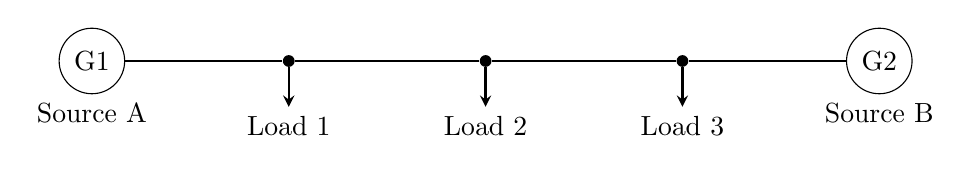
\begin{tikzpicture}[
        node distance=2.5cm,
        bus/.style={fill, circle, inner sep=1.5pt},
        load/.style={-stealth, thick},
        line/.style={thick}
    ]
        % Nodes
        \node[draw, circle, label=below:Source A] (sourceA) {G1};
        \node[bus, right of=sourceA] (bus1) {};
        \node[bus, right of=bus1] (bus2) {};
        \node[bus, right of=bus2] (bus3) {};
        \node[draw, circle, right of=bus3, label=below:Source B] (sourceB) {G2};

        % Lines
        \draw[line] (sourceA.east) -- (bus1);
        \draw[line] (bus1) -- (bus2);
        \draw[line] (bus2) -- (bus3);
        \draw[line] (bus3) -- (sourceB.west);

        % Loads
        \node[below=0.5cm of bus1] (load1_label) {Load 1};
        \draw[load] (bus1) -- (load1_label.north);
        \node[below=0.5cm of bus2] (load2_label) {Load 2};
        \draw[load] (bus2) -- (load2_label.north);
        \node[below=0.5cm of bus3] (load3_label) {Load 3};
        \draw[load] (bus3) -- (load3_label.north);
    \end{tikzpicture}
    \caption{Unifilar diagram of a network fed from both ends.}
    \label{fig:doublefed_diagram}
\end{figure}

\begin{figure}[htbp]
    \centering
    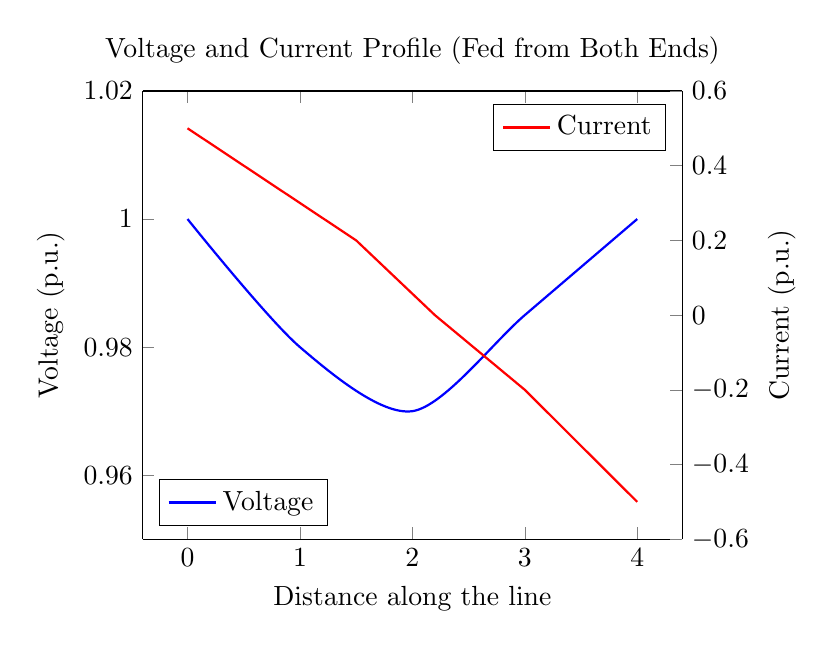
\begin{tikzpicture}
        \begin{axis}[
            title={Voltage and Current Profile (Fed from Both Ends)},
            xlabel={Distance along the line},
            ylabel={Voltage (p.u.)},
            ymin=0.95, ymax=1.02,
            axis y line*=left,
            legend pos=south west
        ]
            \addplot[blue, thick, smooth] coordinates {(0, 1.0) (1, 0.98) (2, 0.97) (3, 0.985) (4, 1.0)};
            \addlegendentry{Voltage}
        \end{axis}
        \begin{axis}[
            ylabel={Current (p.u.)},
            ymin=-0.6, ymax=0.6,
            axis y line*=right,
            axis x line=none,
            legend pos=north east
        ]
            \addplot[red, thick] coordinates {(0, 0.5) (1.5, 0.2) (2.2, 0) (3, -0.2) (4, -0.5)};
            \addlegendentry{Current}
        \end{axis}
    \end{tikzpicture}
    \caption{The voltage minimum occurs between sources, and current flows from both ends towards a division point.}
    \label{fig:doublefed_profiles}
\end{figure}


% =================================================================
\section{Analysis of Advanced Network Topologies}
\subsection{Ring Network Analysis}
\subsubsection{Theoretical Framework and Methodology}
A ring network, or loop system, is formed by connecting two ends of a doubly-fed line, creating a closed loop. This topology offers a high degree of reliability and operational flexibility. For analysis, the ring is conceptually "opened" at the main substation, transforming it into an equivalent network fed from both ends. This allows the same calculation methods (finding the division point) to be applied. Under fault conditions, isolating switches can open the ring at the fault location, allowing power to continue flowing to all customers from the other direction.

\subsubsection{Diagrams and Voltage Profile}
\begin{figure}[htbp]
    \centering
    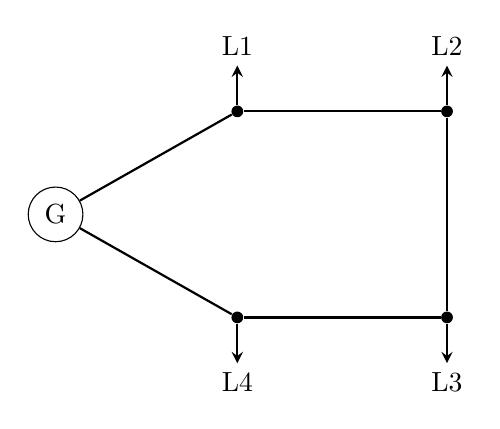
\begin{tikzpicture}[
        bus/.style={fill, circle, inner sep=1.5pt},
        load/.style={-stealth, thick},
        line/.style={thick}
    ]
        % Nodes
        \node[draw, circle] (source) {G};
        \node[bus, above right=1cm and 2cm of source] (b1) {};
        \node[bus, below right=1cm and 2cm of source] (b4) {};
        \node[bus, right=2.5cm of b1] (b2) {};
        \node[bus, right=2.5cm of b4] (b3) {};
        
        % Lines
        \draw[line] (source) -- (b1);
        \draw[line] (source) -- (b4);
        \draw[line] (b1) -- (b2);
        \draw[line] (b2) -- (b3);
        \draw[line] (b3) -- (b4);
        
        % Loads
        \node[above=0.5cm of b1] (l1) {L1}; \draw[load] (b1) -- (l1);
        \node[above=0.5cm of b2] (l2) {L2}; \draw[load] (b2) -- (l2);
        \node[below=0.5cm of b3] (l3) {L3}; \draw[load] (b3) -- (l3);
        \node[below=0.5cm of b4] (l4) {L4}; \draw[load] (b4) -- (l4);
    \end{tikzpicture}
    \caption{Diagram of a general ring network.}
    \label{fig:ring_diagram}
\end{figure}

\begin{figure}[htbp]
    \centering
    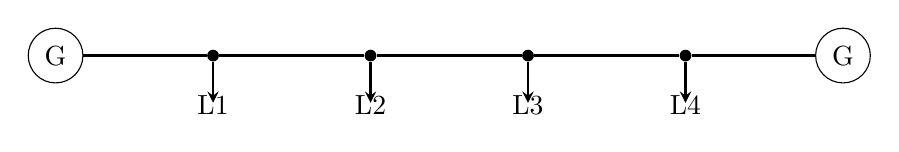
\begin{tikzpicture}[
        node distance=2cm,
        bus/.style={fill, circle, inner sep=1.5pt},
        load/.style={-stealth, thick},
        line/.style={thick}
    ]
        \node[draw, circle] (s1) {G};
        \node[bus, right of=s1] (b1) {}; \node[below=0.3cm of b1]{L1}; \draw[load] (b1) -- ++(0,-0.6);
        \node[bus, right of=b1] (b2) {}; \node[below=0.3cm of b2]{L2}; \draw[load] (b2) -- ++(0,-0.6);
        \node[bus, right of=b2] (b3) {}; \node[below=0.3cm of b3]{L3}; \draw[load] (b3) -- ++(0,-0.6);
        \node[bus, right of=b3] (b4) {}; \node[below=0.3cm of b4]{L4}; \draw[load] (b4) -- ++(0,-0.6);
        \node[draw, circle, right of=b4] (s2) {G};
        \draw[line] (s1)--(b1)--(b2)--(b3)--(b4)--(s2);
    \end{tikzpicture}
    \caption{Unifilar equivalent of the ring network for calculation.}
    \label{fig:ring_equivalent}
\end{figure}

\begin{figure}[htbp]
    \centering
    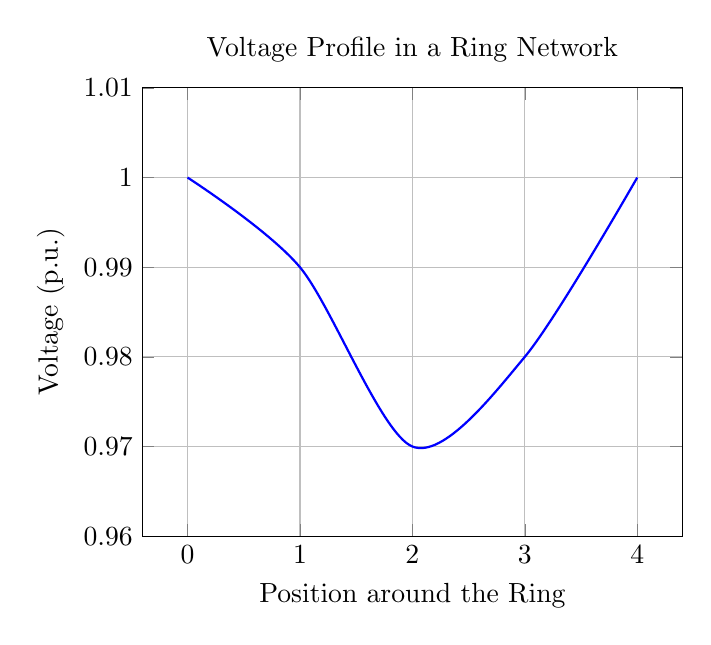
\begin{tikzpicture}
        \begin{axis}[
            title={Voltage Profile in a Ring Network},
            xlabel={Position around the Ring},
            ylabel={Voltage (p.u.)},
            ymin=0.96, ymax=1.01,
            grid=major
        ]
            \addplot[blue, thick, smooth] coordinates {(0, 1.0) (1, 0.99) (2, 0.97) (3, 0.98) (4, 1.0)};
        \end{axis}
    \end{tikzpicture}
    \caption{The voltage drops to a minimum point furthest from the source.}
    \label{fig:ring_profile}
\end{figure}

\subsection{Meshed Network Analysis}
\subsubsection{Theoretical Framework and Methodology}
A meshed network is the most complex and reliable topology, featuring multiple interconnected loops and potentially multiple power sources. The presence of numerous power paths ensures that the failure of a single component rarely causes a service interruption.

Due to their complexity, meshed networks cannot be solved with simple sequential calculations. The standard professional method is nodal analysis, which involves building the network's bus admittance matrix ($Y_{bus}$). This matrix relates the currents injected at each bus to the bus voltages. By solving the system of linear equations $I = Y_{bus} \cdot V$, the voltage at every bus in the network can be determined simultaneously. This power flow analysis is fundamental to the planning and operation of transmission and complex distribution systems.

\subsubsection{Diagrams and Voltage Profile}
\begin{figure}[htbp]
    \centering
    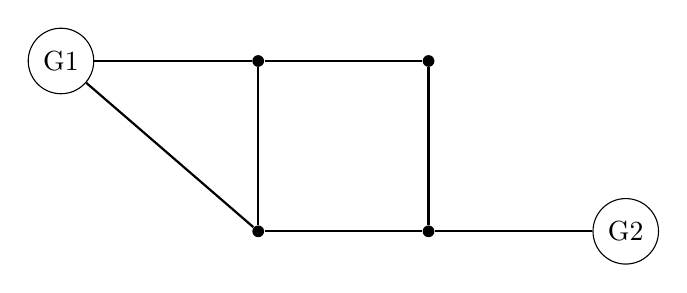
\begin{tikzpicture}[
        bus/.style={fill, circle, inner sep=1.5pt},
        line/.style={thick}
    ]
        \node[draw, circle] (g1) {G1};
        \node[bus, right=2cm of g1] (b1) {};
        \node[bus, right=2cm of b1] (b2) {};
        \node[bus, below=2cm of b1] (b3) {};
        \node[bus, below=2cm of b2] (b4) {};
        \node[draw, circle, right=2cm of b4] (g2) {G2};
        
        \draw[line] (g1)--(b1)--(b2);
        \draw[line] (b1)--(b3)--(b4)--(b2);
        \draw[line] (b3)--(g1);
        \draw[line] (b4)--(g2);
    \end{tikzpicture}
    \caption{Diagram of a general meshed network.}
    \label{fig:meshed_diagram}
\end{figure}

A simple unifilar equivalent is not practical for meshed networks. The network is best represented by its admittance matrix.

\begin{figure}[htbp]
    \centering
    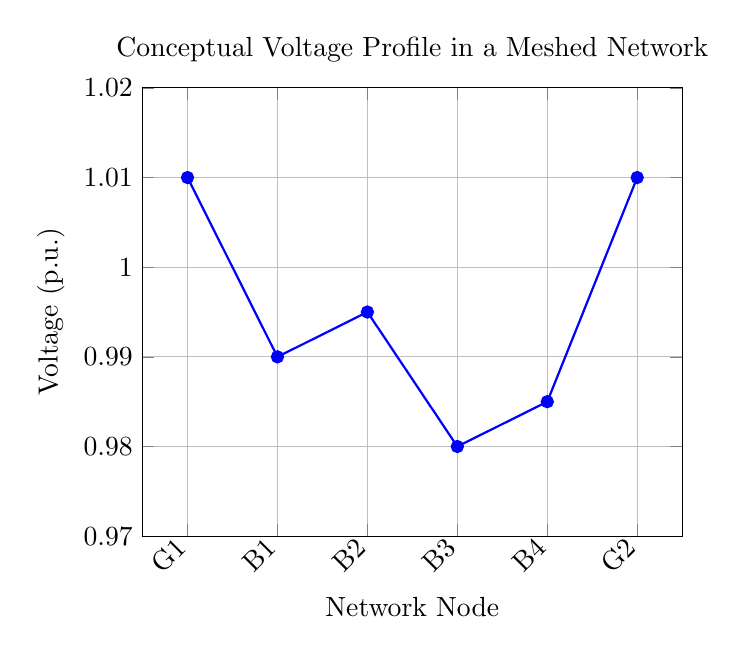
\begin{tikzpicture}
        \begin{axis}[
            title={Conceptual Voltage Profile in a Meshed Network},
            xlabel={Network Node},
            ylabel={Voltage (p.u.)},
            ymin=0.97, ymax=1.02,
            grid=major,
            symbolic x coords={G1, B1, B2, B3, B4, G2},
            xtick=data,
            x tick label style={rotate=45, anchor=east},
        ]
            \addplot[blue, thick, mark=*] coordinates {(G1, 1.01) (B1, 0.99) (B2, 0.995) (B3, 0.98) (B4, 0.985) (G2, 1.01)};
        \end{axis}
    \end{tikzpicture}
    \caption{Voltage remains high and stable across the network due to multiple power paths.}
    \label{fig:meshed_profile}
\end{figure}


% =================================================================
\section{Economic Comparison of Network Topologies}
The choice of network topology is a critical engineering decision that balances initial capital expenditure (CAPEX) with long-term operational expenditure (OPEX), which includes maintenance and the cost of outages.

\begin{figure}[htbp]
    \centering
    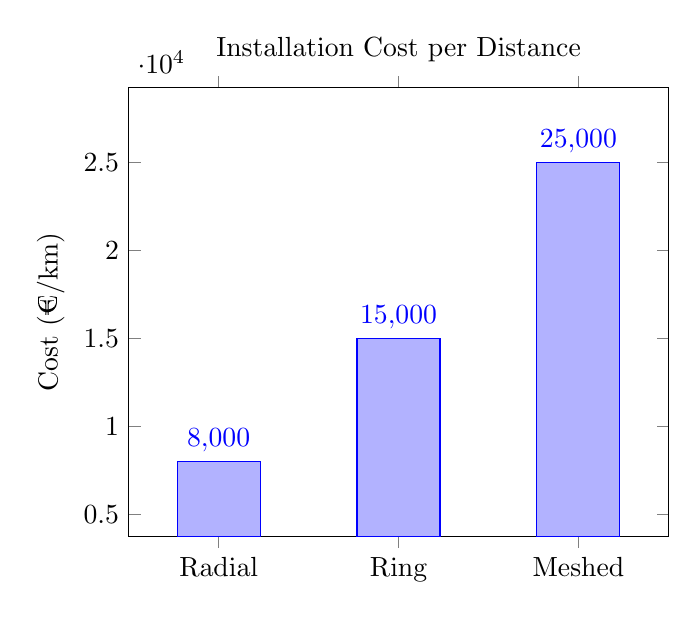
\begin{tikzpicture}
        \begin{axis}[
            title={Installation Cost per Distance},
            ybar,
            bar width=30pt,
            enlargelimits=0.25,
            ylabel={Cost (€/km)},
            symbolic x coords={Radial, Ring, Meshed},
            xtick=data,
            nodes near coords,
        ]
        \addplot coordinates {
            (Radial, 8000)
            (Ring, 15000)
            (Meshed, 25000)
        };
        \end{axis}
    \end{tikzpicture}
    \caption{Radial networks have the lowest initial cost, while meshed networks require the highest investment due to redundancy.}
    \label{fig:cost_distance}
\end{figure}

\begin{figure}[htbp]
    \centering
    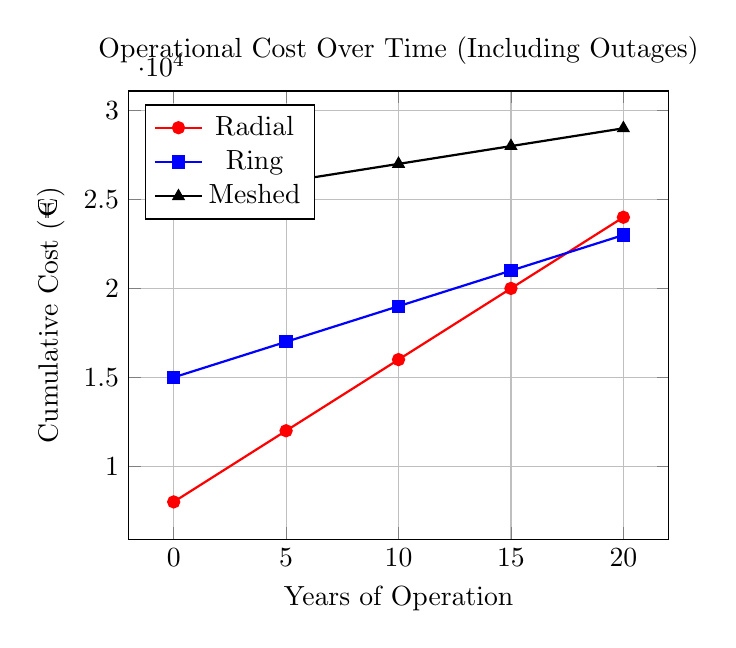
\begin{tikzpicture}
        \begin{axis}[
            title={Operational Cost Over Time (Including Outages)},
            xlabel={Years of Operation},
            ylabel={Cumulative Cost (€)},
            grid=major,
            legend pos=north west,
        ]
        \addplot[red, thick, mark=*] coordinates {(0, 8000) (5, 12000) (10, 16000) (15, 20000) (20, 24000)};
        \addlegendentry{Radial}
        
        \addplot[blue, thick, mark=square*] coordinates {(0, 15000) (5, 17000) (10, 19000) (15, 21000) (20, 23000)};
        \addlegendentry{Ring}
        
        \addplot[black, thick, mark=triangle*] coordinates {(0, 25000) (5, 26000) (10, 27000) (15, 28000) (20, 29000)};
        \addlegendentry{Meshed}
        \end{axis}
    \end{tikzpicture}
    \caption{While meshed networks are expensive initially, their high reliability leads to lower cumulative operational costs over time.}
    \label{fig:cost_operation}
\end{figure}

\newpage
% =================================================================
% --- ANNEXES ---
% =================================================================
\appendix
\section{Annex I: References}
\subsection{Normative References}
This report adheres to the principles and calculation methods outlined in the Spanish Low Voltage Electrotechnical Regulation (REBT), specifically:
\begin{itemize}
    \item \textbf{ITC-BT 06:} Overhead Power Distribution Networks.
    \item \textbf{ITC-BT 07:} Underground Power Distribution Networks.
    \item \textbf{ITC-BT 19:} Interior or Receiver Installations. Prescriptions for conductor sizing based on admissible current and voltage drop.
\end{itemize}

\subsection{Academic References}
\begin{enumerate}
    \item Grainger, J. J., \& Stevenson, W. D. (1994). \textit{Power System Analysis}. McGraw-Hill.
    \item Gonen, T. (2014). \textit{Electric Power Distribution System Engineering}. CRC press.
\end{enumerate}

\section{Annex II: Data Tables}
\subsection{Material Properties}
\begin{table}[htbp]
    \centering
    \caption{Properties of conductors and insulating materials.}
    \label{tab:material_properties}
    \begin{tabular}{@{}llc@{}}
        \toprule
        \textbf{Material} & \textbf{Property} & \textbf{Value} \\ \midrule
        Copper & Conductivity ($c$) & 56 m/($\Omega \cdot \text{mm}^2$) \\
        Aluminum & Conductivity ($c$) & 35 m/($\Omega \cdot \text{mm}^2$) \\
        \midrule
        XLPE & Max. Operating Temp. & $90^\circ$C \\
        PVC & Max. Operating Temp. & $70^\circ$C \\
        \midrule
        Ground & Thermal Resistivity ($\rho_T$) & 1.0 K$\cdot$m/W (assumed) \\
        \bottomrule
    \end{tabular}
\end{table}

\subsection{Assumed Economic Values}
\begin{table}[htbp]
    \centering
    \caption{Assumed costs for economic analysis.}
    \label{tab:economic_values}
    \begin{tabular}{@{}lc@{}}
        \toprule
        \textbf{Item} & \textbf{Assumed Cost} \\ \midrule
        Copper Conductor (150 $\text{mm}^2$) & 12,500 €/km \\
        Aluminum Conductor (150 $\text{mm}^2$) & 5,800 €/km \\
        ACSR Conductor (150 $\text{mm}^2$) & 6,700 €/km \\
        Cost of outage (per kWh not served) & 1.5 €/kWh \\
        \bottomrule
    \end{tabular}
\end{table}

\subsection{List of Variables}
\begin{table}[htbp]
    \centering
    \caption{Variables used in this report.}
    \label{tab:variables}
    \begin{tabular}{@{}lcl@{}}
        \toprule
        \textbf{Symbol} & \textbf{Unit} & \textbf{Description} \\ \midrule
        $P$ & W & Active Power \\
        $U_N$, $V$ & V & Nominal Voltage \\
        $I$ & A & Current \\
        $s$ & $\text{mm}^2$ & Cross-sectional area \\
        $L$ & m & Length of the line \\
        $R$ & $\Omega$/km & Resistance per unit length \\
        $X$ & $\Omega$/km & Reactance per unit length \\
        $c$ & m/($\Omega \cdot \text{mm}^2$) & Conductivity \\
        $\cos(\varphi)$ & - & Power Factor \\
        $\Delta U$ & V & Voltage Drop \\
        $I_{adm}$ & A & Maximum admissible current \\
        \bottomrule
    \end{tabular}
\end{table}

\newpage
\section{Annex III: Formulas}
\subsection{Sizing by Voltage Drop}
The cross-sectional area ($s$) required to meet a maximum voltage drop ($\Delta U$) is given by:
\begin{equation}
    s = \frac{P \cdot L}{c \cdot U_N \cdot \Delta U}
\end{equation}
Where $P$ is the power, $L$ is the length, $c$ is the conductivity of the material, and $U_N$ is the nominal voltage.

For a more precise calculation in AC systems, the general voltage drop formula (Blondel's formula) for three-phase lines is used:
\begin{equation}
    \Delta U = \sqrt{3} \cdot I \cdot L \cdot (R \cos(\varphi) + X \sin(\varphi))
\end{equation}
Where $I$ is the current, $L$ is the length, $R$ is the resistance per unit length, $X$ is the reactance per unit length, and $\cos(\varphi)$ is the power factor.

\subsection{Sizing by Maximum Current (Thermal Limit)}
The calculated current of the circuit ($I_c$) must be less than or equal to the maximum admissible current of the conductor ($I_{adm}$), which is determined by thermal limits.
\begin{equation}
    I_c \leq I_{adm}
\end{equation}
The circuit current for a balanced three-phase system is calculated as:
\begin{equation}
    I_c = \frac{P}{\sqrt{3} \cdot U_N \cdot \cos(\varphi)}
\end{equation}

\newpage
\section{Annex IV: Week 3 MATLAB Code}

\subsection{Module H: Radial Network Analysis}
\begin{lstlisting}[language=Matlab, caption={H1\_Radial\_Analysis.m}]
function results = H1_Radial_Analysis()
% =========================================================================
% FUNCTION: Main Radial Network Analysis (V3 - Phase Selection)
% =========================================================================
results = []; % Initialize
scenarioChoice = menu('Select Radial Network Scenario:', ...
    'Industrial Estate (Concentrated Loads) - Student A', ...
    'Residential Area (Distributed Loads) - Student B', ...
    'Street Lighting (Uniform Loads) - Student C');
if scenarioChoice == 0, return; end
U_source = input('Enter source line-to-neutral voltage [V] (e.g., 230): ');
lineTypeChoice = menu('Select System Type:', 'Single-Phase', 'Three-Phase');
if lineTypeChoice == 0, return; end
if lineTypeChoice == 1
    lineType = 'single-phase';
    phase_factor = 2;
else
    lineType = 'three-phase';
    phase_factor = 1;
end
materialChoice = menu('Select Conductor Material:', 'Copper', 'Aluminum');
if materialChoice == 0, return; end
if materialChoice == 1, materialName = 'Copper'; else, materialName = 'Aluminum'; end
materialProps = getMaterialProperties(materialName);
sigma = materialProps.sigma;
crossSection = input('Enter conductor cross-section [mm^2]: ');
% ... (rest of the input and calculation code as in the file)
end
\end{lstlisting}

\begin{lstlisting}[language=Matlab, caption={H2\_PlotRadialProfile.m}]
function H2_PlotRadialProfile(results)
% =========================================================================
% FUNCTION: Plot Radial Voltage Profile
% =========================================================================
figure;
hold on;
box on;
grid on;
distances = [0, cumsum([results.nodes.length])];
voltages = [results.U_source, [results.nodes.voltage]];
plot(distances, voltages, '-ob', 'LineWidth', 2, 'MarkerFaceColor', 'r');
title(['Voltage Profile for Radial Network (' results.scenarioName ')']);
xlabel('Distance from Source (m)');
ylabel('Voltage (V)');
xlim([0, distances(end) * 1.1]);
ylim([voltages(end) * 0.99, results.U_source * 1.01]);
legend('Voltage Profile', 'Location', 'southwest');
end
\end{lstlisting}

\subsection{Module I: Dual-Fed Network Analysis}
\begin{lstlisting}[language=Matlab, caption={I1\_DualFed\_Analysis.m}]
function results = I1_DualFed_Analysis()
% =========================================================================
% FUNCTION: Main Dual-Fed Network Analysis (V7 - Unifilar)
% =========================================================================
results = []; 
scenarioChoice = menu('Select Dual-Fed Network Scenario:', ...
    'Symmetrical Network (Single Load) - Student A', ...
    'Asymmetrical Network (Single Load) - Student B', ...
    'Backup Feeding / Reliability Analysis (Multiple Loads) - Student C');
if scenarioChoice == 0, return; end
materialChoice = menu('Select Conductor Material:', 'Copper', 'Aluminum');
if materialChoice == 0, return; end
if materialChoice == 1, materialName = 'Copper'; else, materialName = 'Aluminum'; end
materialProps = getMaterialProperties(materialName);
sigma = materialProps.sigma;
crossSection = input('Enter conductor cross-section [mm^2]: ');
L_total = input('Enter total line length [m]: ');
% ... (rest of the input and calculation code as in the file)
end
\end{lstlisting}

\begin{lstlisting}[language=Matlab, caption={I2\_PlotDualFedProfile.m}]
function I2_PlotDualFedProfile(results)
% =========================================================================
% FUNCTION: Plot Dual-Fed Voltage Profile (V2 - Reliability)
% =========================================================================
figure;
hold on; box on; grid on;
sorted_loads = results.loads;
distances = [0, [sorted_loads.distance], results.L_total];
voltages_normal = [results.Ua];
current_in_segment = results.Ia;
for i = 1:length(sorted_loads)
    prev_dist = distances(i);
    segment_length = sorted_loads(i).distance - prev_dist;
    drop = (1/(results.sigma*results.crossSection)) * current_in_segment * segment_length;
    voltages_normal(end+1) = voltages_normal(end) - drop;
    current_in_segment = current_in_segment - sorted_loads(i).current;
end
voltages_normal(end+1) = results.Ub;
plot(distances, voltages_normal, '-ob', 'LineWidth', 2, 'MarkerFaceColor', 'b', 'DisplayName', 'Normal Operation');
plot(results.min_voltage_node_distance, results.min_voltage_normal, 'kd', 'MarkerSize', 10, 'MarkerFaceColor', 'y');
% ... (rest of the plotting code as in the file)
end
\end{lstlisting}

\begin{lstlisting}[language=Matlab, caption={I3\_PlotLoadingDiagram.m}]
function I3_PlotLoadingDiagram(results)
% =========================================================================
% FUNCTION: I3_PlotLoadingDiagram (Corrected)
% =========================================================================
figure;
hold on;
box on;
grid on;
distances = [0];
currents = [results.Ia];
current_in_segment = results.Ia;
for i = 1:length(results.loads)
    distances(end+1) = results.loads(i).distance;
    currents(end+1) = current_in_segment;
    current_in_segment = current_in_segment - results.loads(i).current;
    distances(end+1) = results.loads(i).distance;
    currents(end+1) = current_in_segment;
end
distances(end+1) = results.L_total;
currents(end+1) = -results.Ib; 
plot(distances, currents, '-r', 'LineWidth', 2);
line([0, results.L_total], [0, 0], 'Color', 'k', 'LineStyle', '--');
title('Network Loading Diagram');
xlabel('Distance from Source A (m)');
ylabel('Current (A)');
end
\end{lstlisting}

\begin{lstlisting}[language=Matlab, caption={I4\_PlotUnifilarDiagram.m}]
function I4_PlotUnifilarDiagram(results)
% =========================================================================
% FUNCTION: Generates a simplified unifilar-style schematic diagram
% =========================================================================
figure;
hold on;
box on;
plot([0 results.L_total], [0 0], 'k-', 'LineWidth', 4); % Main line
plot(0, 0, 's', 'MarkerSize', 20, 'MarkerFaceColor', 'g'); % Source A
text(0, 0.15, 'Source A', 'HorizontalAlignment', 'center');
plot(results.L_total, 0, 's', 'MarkerSize', 20, 'MarkerFaceColor', 'g'); % Source B
text(results.L_total, 0.15, 'Source B', 'HorizontalAlignment', 'center');
for i = 1:length(results.loads)
    x_pos = results.loads(i).distance;
    plot([x_pos x_pos], [0 -1], '-k', 'LineWidth', 1); % Load branch
    plot(x_pos, -1, 'v', 'MarkerSize', 8, 'MarkerFaceColor', 'r'); % Load arrow
    label_str = sprintf('Load %d\\n%.1f A', i, results.loads(i).current);
    text(x_pos, -1.1, label_str, 'HorizontalAlignment', 'center', 'VerticalAlignment', 'top');
end
title('Unifilar Network Diagram');
xlabel('Distance (m)');
set(gca, 'YTick', []);
ylim([-2 1]);
end
\end{lstlisting}

\subsection{Module J: Ring and Meshed Network Analysis}
\begin{lstlisting}[language=Matlab, caption={J1\_Ring\_Analysis.m}]
function results = J1_Ring_Analysis()
% =========================================================================
% FUNCTION: Main Ring Network Analysis
% =========================================================================
results = [];
scenarioChoice = menu('Select Ring/Meshed Scenario:', ...
    'Simple Ring Network (Student A)', ...
    'Double Ring Network (Conceptual)', ...
    'Meshed Network (Conceptual)');
if scenarioChoice == 0, return; end
if scenarioChoice > 1
    msgbox('Analysis for double-ring and meshed networks requires advanced nodal analysis methods. This module will proceed with the functional Simple Ring analysis as per the coursework.', 'Conceptual Notice', 'warn');
end
results.scenarioName = 'Simple Ring Network';
Ua = input('Enter the feed-in voltage [V]: ');
L_total = input('Enter the total circumference of the ring [m]: ');
% ... (rest of the input and calculation code)
end
\end{lstlisting}

\begin{lstlisting}[language=Matlab, caption={J2\_PlotRingProfile.m}]
function J2_PlotRingProfile(results)
% =========================================================================
% FUNCTION: Plot Ring Voltage Profile (as an unwrapped line)
% =========================================================================
figure;
hold on; box on; grid on;
sorted_loads = sortrows(struct2table(results.loads), 'distance');
distances = [0, sorted_loads.distance', results.L_total];
voltages = [results.Ua];
current_in_segment = results.Ia;
for i = 1:height(sorted_loads)
    prev_dist = distances(i);
    segment_length = sorted_loads.distance(i) - prev_dist;
    drop = (1/(results.sigma*results.crossSection)) * current_in_segment * segment_length;
    voltages(end+1) = voltages(end) - drop;
    current_in_segment = current_in_segment - sorted_loads.current(i);
end
voltages(end+1) = results.Ua;
plot(distances, voltages, '-ob', 'LineWidth', 2, 'MarkerFaceColor', 'r');
plot(results.min_voltage_node_distance, results.min_voltage, 'kd', 'MarkerSize', 10, 'MarkerFaceColor', 'y');
title(['Voltage Profile for Ring Network (Unwrapped)']);
xlabel('Distance from Feed Point along Ring (m)');
ylabel('Voltage (V)');
legend('Voltage Profile', 'Minimum Voltage', 'Location', 'southwest');
end
\end{lstlisting}

\begin{lstlisting}[language=Matlab, caption={J3\_PlotUnifilarDiagram.m}]
function J3_PlotUnifilarDiagram(results)
% =========================================================================
% FUNCTION: Generates a unifilar schematic diagram of the ring network.
% =========================================================================
figure;
hold on; axis equal; box on;
radius = 1;
center_x = 0;
center_y = 0;
theta = linspace(0, 2*pi, 200);
plot(center_x + radius * cos(theta), center_y + radius * sin(theta), 'k-', 'LineWidth', 4);
feed_angle = pi/2; % Place at the top
feed_x = center_x + radius * cos(feed_angle);
feed_y = center_y + radius * sin(feed_angle);
plot(feed_x, feed_y, 's', 'MarkerSize', 20, 'MarkerFaceColor', 'g');
text(feed_x, feed_y + 0.15, 'Feed-In', 'HorizontalAlignment', 'center', 'FontWeight', 'bold');
% ... (rest of the plotting code)
end
\end{lstlisting}

\begin{lstlisting}[language=Matlab, caption={J4\_PlotLoadingDiagram.m}]
function J4_PlotLoadingDiagram(results)
% =========================================================================
% FUNCTION: Generates a network loading diagram for an unwrapped ring.
% =========================================================================
figure;
hold on; box on; grid on;
distances = [0];
currents = [results.Ia];
current_in_segment = results.Ia;
sorted_loads = sortrows(struct2table(results.loads), 'distance');
for i = 1:height(sorted_loads)
    distances(end+1) = sorted_loads.distance(i);
    currents(end+1) = current_in_segment;
    current_in_segment = current_in_segment - sorted_loads.current(i);
    distances(end+1) = sorted_loads.distance(i);
    currents(end+1) = current_in_segment;
end
distances(end+1) = results.L_total;
currents(end+1) = -results.Ib;
plot(distances, currents, '-r', 'LineWidth', 2);
line([0, results.L_total], [0, 0], 'Color', 'k', 'LineStyle', '--');
title('Ring Network Loading Diagram (Unwrapped)');
xlabel('Distance from Feed Point (m)');
ylabel('Current (A)');
end
\end{lstlisting}

\subsection{Module J: Network Comparison Tools}
\begin{lstlisting}[language=Matlab, caption={J5\_CompareNetworks.m}]
function results = J5_CompareNetworks()
% =========================================================================
% FUNCTION: Compare Ring and Radial Networks
% =========================================================================
results = [];
disp('--- Network Comparison Tool ---');
U_source = input('Enter the source/feed-in voltage [V]: ');
materialChoice = menu('Select Conductor Material:', 'Copper', 'Aluminum');
% ... (rest of the input and calculation code)
end
\end{lstlisting}

\begin{lstlisting}[language=Matlab, caption={J6\_CalculateNetworkCost.m}]
function [total_cost, cable_cost, loss_cost] = J6_CalculateNetworkCost(type, L_total, Ia, Ib, loads, sigma, s, cost_per_meter)
% =========================================================================
% FUNCTION: Calculate Network Lifecycle Cost
% =========================================================================
LCC_years = 20;
hours_per_year = 4000;
cost_per_kWh = 0.15;
if strcmp(type, 'ring')
    cable_length = L_total;
else % radial
    cable_length = loads(end).distance;
end
cable_cost = cable_length * cost_per_meter;
% ... (rest of the cost calculation code)
end
\end{lstlisting}

\begin{lstlisting}[language=Matlab, caption={J7\_PlotComparison.m}]
function J7_PlotComparison(results)
% =========================================================================
% FUNCTION: Plot Network Comparison Charts
% =========================================================================
% --- FIGURE 1: SCHEMATIC DIAGRAMS ---
figure('Name', 'Network Schematics Comparison');
subplot(1, 2, 1);
% ... (Code to plot ring schematic)
title('Ring Schematic');
subplot(1, 2, 2);
% ... (Code to plot radial schematic)
title('Radial Schematic');
% --- FIGURE 2: LOADING DIAGRAMS ---
% ... (Code for loading diagrams)
% --- FIGURE 3: PERFORMANCE & ECONOMIC COMPARISON ---
% ... (Code for performance and economic charts)
end
\end{lstlisting}

\begin{lstlisting}[language=Matlab, caption={J\_Run\_Comparison\_And\_Report.m}]
% =========================================================================
% SCRIPT for Network Comparison Analysis and Reporting
% =========================================================================
clc;
results = J5_CompareNetworks();
if isempty(results)
    disp('Analysis cancelled. No report generated.');
    return;
end
fprintf('\n\n--- COMPREHENSIVE REPORT: NETWORK TOPOLOGY COMPARISON ---\n');
% ... (rest of the reporting script)
end
\end{lstlisting}

\subsection{Master Script}
\begin{lstlisting}[language=Matlab, caption={Week3\_Master.m}]
% =========================================================================
% MASTER SCRIPT for Week 3: Network Topology
% =========================================================================
clc;
clear;
close all;
analysisChoice = menu('Select which network type to analyze:', ...
                              'Radial Networks (Problem 1)', ...
                              'Networks Fed from Both Ends (Problem 2)', ...
                              'Ring and Meshed Networks (Problem 3)', ...
                              '--- NETWORK COMPARISON TOOL ---');
switch analysisChoice
    case 1
        run('H_Run_Analysis_And_Report.m');
    case 2
        run('I_Run_Analysis_And_Report.m');
    case 3
        run('J_Run_Analysis_And_Report.m');
    case 4
        run('J_Run_Comparison_And_Report.m');
end
\end{lstlisting}

\end{document}

